%Es hat sich gezeigt, dass mit modernen JavaScript-Entwicklungswerkzeugen 
%auch ohne umfassende Kenntnisse der Softwareentwicklung zugänglich sind.
Es konnte gezeigt werden, wie die Entwicklung einer Webanwendung mit den Technologien des MERN-Stacks erfolgt.
Die Anwendung wurde im Zeitraum von Anfang Mai 2021 bis Mitte August 2021 entwickelt.
Mit grundlegenden Programmierkenntnissen war es möglich, eine funktionelle Anwendung mit einigen Funktionen zu entwicklen.
Diese sind: die Registrierung für neue Benutzer, die Anmeldung für bestehende Benutzer, die Verwaltung deren persönlichen Daten, die Interaktion mit anderen Benutzern auf der Grundlage ihrer Präferenzen und ein auf Textnachrichten basierter Kommunikationskanal.
\\\\
%TInfra
In Kapitel \ref{kap_Technologieinfrastruktur} wurde ein Ausblick auf die Architektur der Anwendung gegeben. %DB
Die Auswahl der Datenbank und deren Schemata wurde in Kapitel \ref{kap_Datenbank} erläutert.
In den Kapitel \ref{kap_Backend} und \ref{kap_Schnittstelle} wurde die Logik erläutert, die benötigt ist, um Daten in der Datenbank auszulesen und zu manipulieren.
Dies geschieht durch eine REST-Schnittstelle für das in Amazon S3 gespeicherten Profilbild und GraphQL-Endpunkte für die Verwaltung von Nutzerdaten. 
%Backend %Schnittstelle 
%Frontend
In Kapitel \ref{kap_Frontend} wird gezeigt, welche Kriterien für die Wahl von React berücksichtigt wurden. 
Außerdem wurde die Entwicklung der Benutzeroberfläche mit React-Hooks gezeigt. 
%Qualitätssicherung
Die Erstellung der Unit- und End-To-End-Tests wie in Kapitel \ref{kap_QS} beschrieben würde die Testzeit für komplexere Anwendungen verringern.
Im Falle des vorliegenden Projekts handelte es sich um ein zusätzliches Werkzeug, dessen Einbindung in den Entwicklungszyklus etwa fünf Tage in Anspruch nahm.
Durch besagte Tests konnten einige Fehler bereits in der Entwicklungszeit korrigiert werden und die Code-Qualität stark erhöht werden.
Bei der Weiterführung des Projekts erhöht sich mit wachsender Komplexität die Wichtigkeit von Testfällen noch weiter.
%Einer signifikante Wert haben die Unit-Test, 
%Was konnte nicht geschafft werden?
\\\\
Der Fokus des Projekts lag darin, eine funktionelle Minimalanwendung zu entwicklen. Es wurde auf Funktionen verzichtet, welche den geplanten Zeitraum des Projekts überschreiten würden.
Für die Weiterentwicklung des Projekts gibt es einige Funktionen, welche sinnvollerweise in das Projekt integriert werden sollten.
Eine Startseite soll einen potenziellen Nutzer einen Einblick in die Anwendung geben.
Um den Einstieg für neue Nutzer noch weiter zu vereinfachen, bietet es sich an, den Login direkt mit Facebook- oder Google-Konto zu ermöglichen.
Für eine bessere Gebrauchlichkeit %Usability
bietet es sich an, neben der Webapplikation eine mobile Applikation zu entwickeln.
Auf Basis der verwendeten Technologien würde sich hierfür React-Native eignen.
Um die Echtheit der Nutzer zu prüfen bietet es sich an, eine Kontovalidierung über die Schnittstelle von \enquote{Riot Games} (Entwickler von \enquote{League of Legends}) einzurichten.
Zum Melden von Nutzern besteht bereits eine Schnittstelle, diese wird vom Frontend jedoch noch nicht angesprochen.
Auch soll ein Algorithmus auf Basis der Meldungen entscheiden, welche Benutzer vom Dienst ausgeschlossen werden.
Es sollten Überlegungen zur Finanzierung aufgestellt werden.
Ein kostenpflichtiges Premium-Abo mit zusätzlichen Funktionen und/oder Bannerwerbung bieten sich an.

\section*{Arbeitsverteilung}

\begin{figure}[h!]
    \centering
    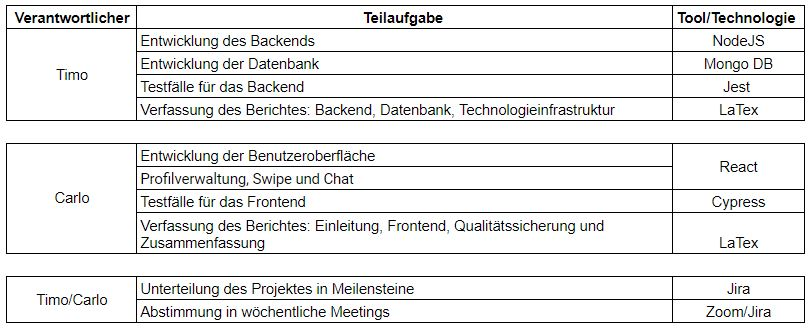
\includegraphics[scale=0.7]{sources/Arbeitsverteilung}
    \caption{Arbeitsverteilung des Projekts. Eigene Darstellung.}
    \label{fig:Antwort_Serverabfrage} 
  \end{figure}